\titleformat % design des titres des chapitres
{\chapter}
[display]
{\centering\normalfont\Large\scshape\bfseries}
{\rule[3pt]{0.15\linewidth}{3pt}\quad\chaptertitlename~\thechapter\quad \rule[3pt] {0.15\linewidth}{3pt}}
{0\baselineskip}%espace vertical entre chapitre et nom du chapitre
{\rule{\linewidth}{0.5pt}\break\Huge}
[\vspace{-0.5\baselineskip}\rule{\linewidth}{0.5pt}\vspace{0\baselineskip}]

\let\clearpage\relax% Stop LaTeX from going to a new page; and
\vspace*{5.5cm}%

\chapter{Context general du projet}
Dans ce premier chapitre, je vais présenter l’entreprise d’accueil
DXC Technology Maroc à travers une description de l’historique ainsi
que son domaine d’activité et l’organigramme puis enfin une
présentation de ses clients.






\newpage
\section{Description générale de DXC Technology Maroc}

Pour définir DXC Technology Maroc il faut tout d’abord définir DXC Technology. \\[0.3cm]
DXC Technology est une multinational de service informatique. Née d'une fusion entre Hewlett Packard Enterprise (HPE) leader mondial de service informatique et Computer Sciences Corporation (CSC) qui gère les métiers du conseil informatique.\\[0.3cm]
DXC Technology Maroc est une co-entreprise entre DXC et la caisse de dépôt et de gestion (CDG) composé de deux sites de production dont le siège se trouve à Sala al Jadida plus précisément à Technopolis ainsi qu’un autre site de production qui se situe à Casa Near shore. DXC Technology Maroc bénéficie de plus de 15 ans d’expérience dans le domaine informatique comptant plus de 1200 collaborateur qui travaille aujourd’hui en deux modes : hybride et distancielle.

\section{Fiche signalétique de l’entreprise :}

Le tableau suivant présente la fiche signalétique de l’entreprise, c’est la carte d’identité de
l’entreprise.

\begin{figure}[h]
    \centering
    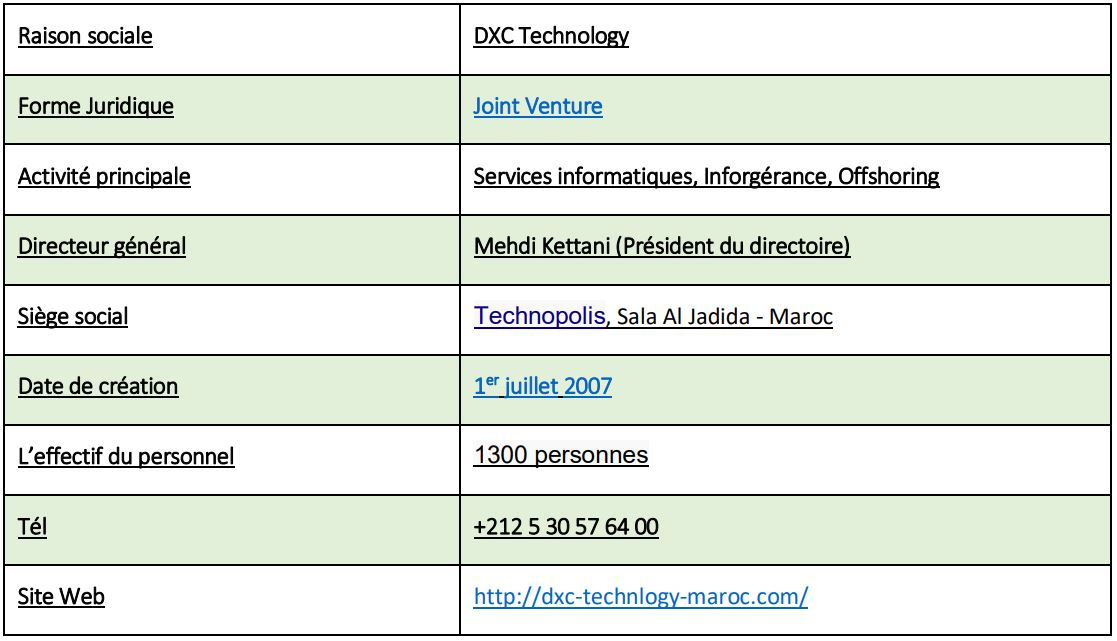
\includegraphics[width=\textwidth]{Rapport de stage PFE chez DXC/figures/fiche_entreprise.jpg}
    \caption{Fiche signalétique de l'entreprise}
\end{figure}

\newpage

\section{Historique et fait Marquants :}

La figure suivante présente l’évolution d’aventure de l’entreprise depuis 2007 jusqu’à 2014.

\begin{figure}[!h]
    \centering
    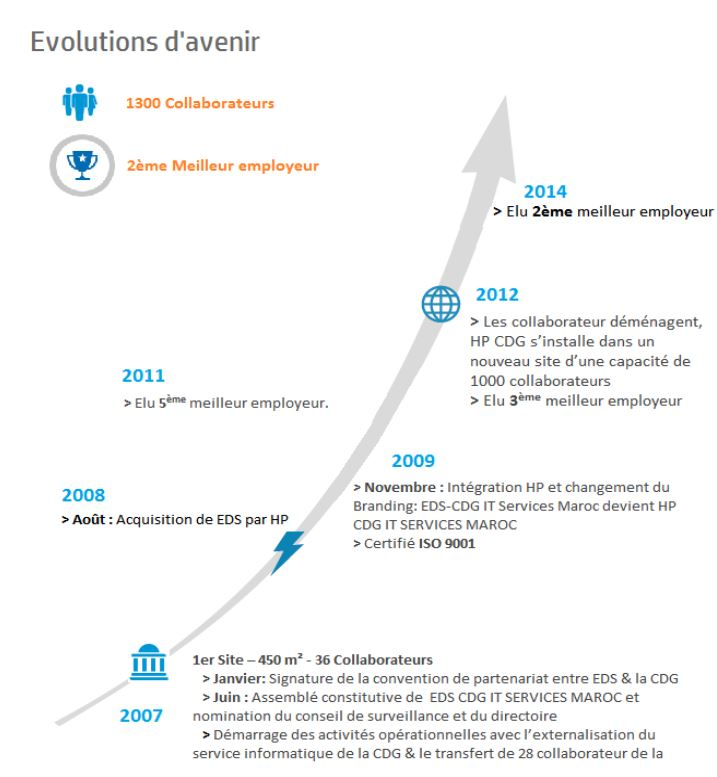
\includegraphics[scale=0.9,keepaspectratio]{Rapport de stage PFE chez DXC/figures/evolution_entreprise.jpg}
    \caption{Evolution de DXC Technology Maroc}
\end{figure}

\newpage

\subsection{Secteurs d’activités :}

DXC Technology est un centre de services qui dispose de ressources compétentes dans les
métiers de services informatiques suivants :

\begin{description}
  \item \textbf{Assurance:} La première mondiale des services et des solutions logicielles pour l’assurance. Soutient la croissance des assureurs, et amélien leur time-to-market et leur excellence opérationnelle grâce à des solutions d’assurance digitale et de gestion déléguée de leurs processus métiers.
  \item \textbf{Sante et Sciences de la vie:} Elle propose des logiciels leaders sur le marché et des services de gestion déléguée (BPS) pour les fournisseurs de soins, les payeurs, l’Etat et les entreprises de soins de santé. Elles se focalisent sur les soins cliniques et l’efficacité opérationnelle avec ses solutions de transformation digitale de soins.
  \item \textbf{Secteur public:} Ils sont un des leaders mondiaux de services informatiques indépendants et travaillent à tous les niveaux (Etat, administrations, collectivistes locales). Ils proposent pour les opérations et systèmes critiques une assistance 24 heures sur 24, et 7 jours sur 7.
  \item \textbf{Énergie:} Depuis plus de 20 ans, ils ont accompagné plus de 400 acteurs du secteur énergétique dans le monde entier. Leurs solutions les aident à saisir rapidement les opportunités du marché, se forger un avantage concurrentiel et mettre en œuvre de nouveaux modèles économiques.
  \item \textbf{Énergie:} Ils sont un desacteurs principaux des services informatiques dédiés aux secteurs Automobile, Équipements industriels, Chimie et High Tech. Ils allaient leurs solides connaissances sectorielles à des expertises spécifiques (Internet des objets, analytique, sécurité) pour aider leurs clients à doper leur innovation.
  \item \textbf{Communication, médias et divertissement:} Ils fournissent des solutions métiers innovantes aux acteurs du secteur Communication, médias et divertissement, aux quatre coins du monde, pour les aider à transformer leur organisation, réenchanter l’expérience client et tirer profit de la convergence digitale.
  \item \textbf{Aéronautique et défense:} Ils sont un des leaders des services informatiques dédiés au secteur Aéronautique et défense. Ils aident leurs clients à raccourcir leur time-to-market, prendre de meilleures décisions en exploitant la richesse de leurs données et adopter les technologies digitales. Ils accélèrent la mise en œuvre de l’innovation sur l’ensemble de la chaîne d’approvisionnement et de fabrication.
  \item \textbf{Transport et tourisme:} Avec plus de 40 ans d’expérience sur le marché, elle soutient les systèmes critiques du secteur (compagnies aériennes, passagers, fret, logistique, entreprises ferroviaires). Ses services aident leurs clients à soutenir leur croissance et les accompagne durant leur transformation.
  \item \textbf{Industrie:} Ils sont un desacteurs principaux des services informatiques dédiés aux secteurs Automobile, Équipements industriels, Chimie et High Tech. Ils allaient leurs solides connaissances sectorielles à des expertises spécifiques (Internet des objets, analytique, sécurité) pour aider leurs clients à doper leur innovation.
  \item \textbf{Distribution et grande consommation:} Ils aident les leaders mondiaux de la distribution et des biens de grande consommation se concentrer sur l’expérience client, et à saisir les opportunités liées aux nouvelles tendances digitales.
  \item \textbf{Communication, médias et divertissement:} Ils fournissent des solutions métiers innovantes aux acteurs du secteur Communication, médias et divertissement, aux quatre coins du monde, pour les aider à transformer leur organisation, réenchanter l’expérience client et tirer profit de la convergence digitale.
  \item \textbf{Aéronautique et défense:}Ils sont un des leaders des services informatiques dédiés au secteur Aéronautique et défense. Ils aident leurs clients à raccourcir leur time-to-market, prendre de meilleures décisions en exploitant la richesse de leurs données et adopter les technologies digitales. Ils accélèrent la mise en œuvre de l’innovation sur l’ensemble de la chaîne d’approvisionnement et de fabrication.
  
\end{description}

\vspace{0.4cm}

\subsection{Les clients de DXC Technologie Maroc :}

La figure suivante présente les différents clients et partenaires commerciaux de DXC.

\vspace{0.3cm}

\begin{figure}[!h]
    \centering
    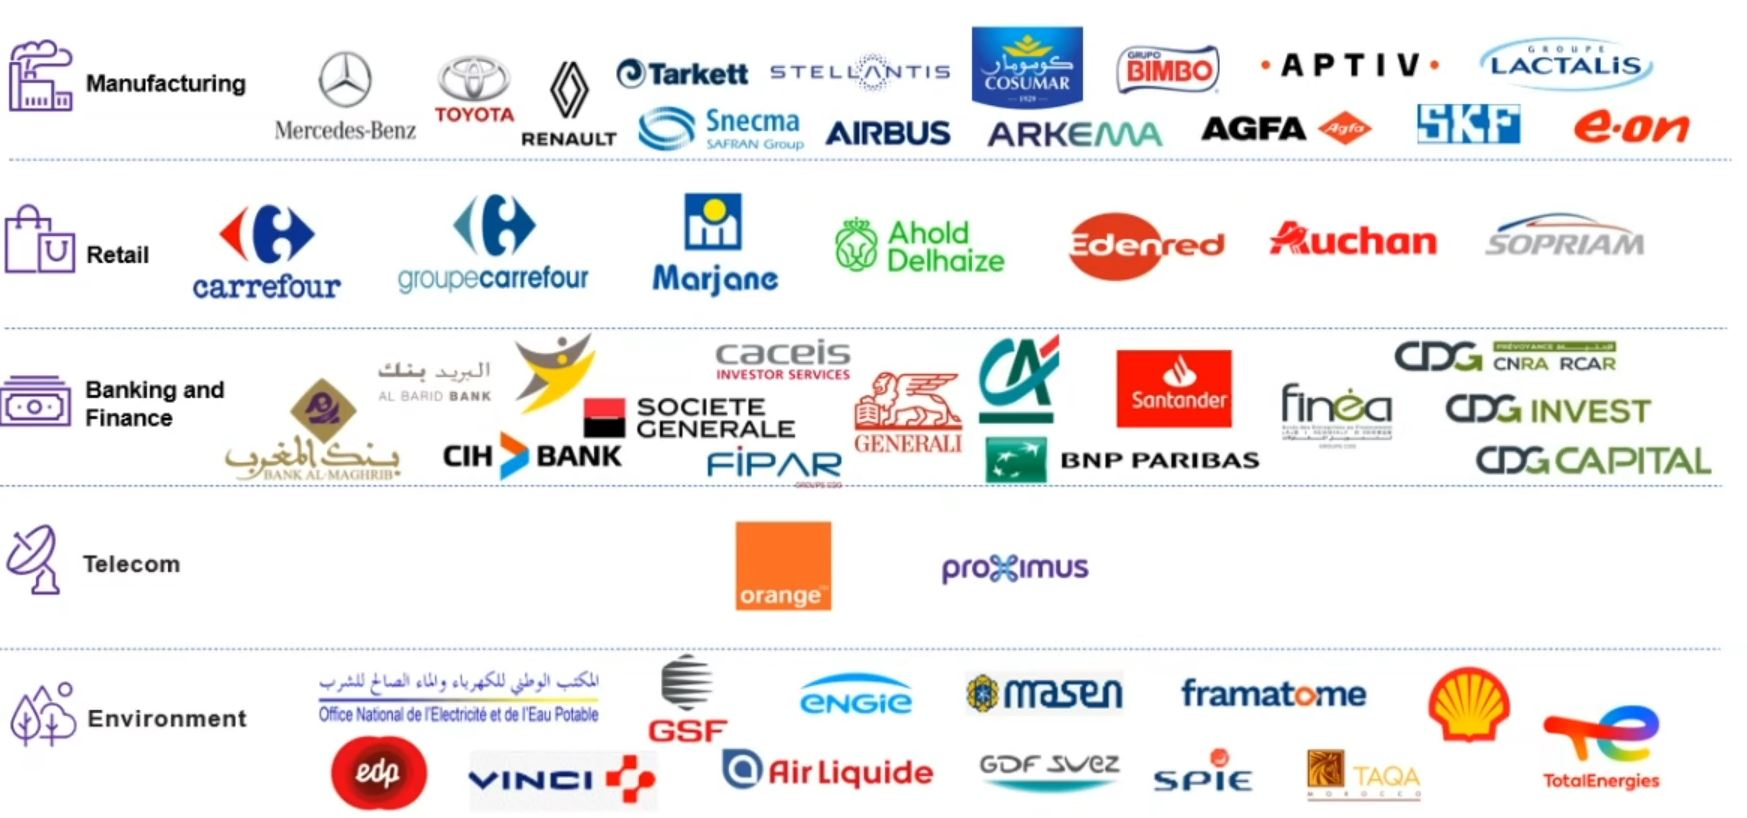
\includegraphics[scale=0.36,keepaspectratio]{Rapport de stage PFE chez DXC/figures/client.jpg}
    \caption{Les clients de DXC Technologie Maroc}
\end{figure}

\newpage

\subsection{Organigramme :}
La figure suivante présente quelques divisions principales de l’entreprise et pas la totalité
des divisions, il est divisé en 2 parties "Support" et "Services Lines" :

\begin{description}
  \item \textbf{Support :} rassemble l’ensemble d'activités de gestion considérées comme ne constituant pas le cœur de métier. Ces activités assurent le fonctionnement de l'entreprise et sont généralement communes à plusieurs divisions ou ligne de produits métier, tel que le service Finance, Ressources Humaines, marketing et service de ventes.
  \item \textbf{Service Lines :} contient les divisions qui représentent le cœur de métier, ces divisons
 sont :
 \begin{enumerate}
   \item \textbf{Application Services :} représente généralement les services de développement informatique et qualité logiciel, ainsi que l’intégration des ERP et le support applicatif.
   \item \textbf{Global Operations Services :} c’est une division dédiée pour les services d’Infrastructure, Cloud et Sécurité des systèmes d’information.
   \item \textbf{Business Process Outsourcing : } l’ensemble des activités qui ont comme but l'externalisation d'une partie de l'activité de l'entreprise vers un prestataire extérieur.
    \item \textbf{MWS  : } assure les services de gestion et support de mobilité, et le support au Delivery.
 \end{enumerate}
  
  \begin{figure}[!h]
    \centering
    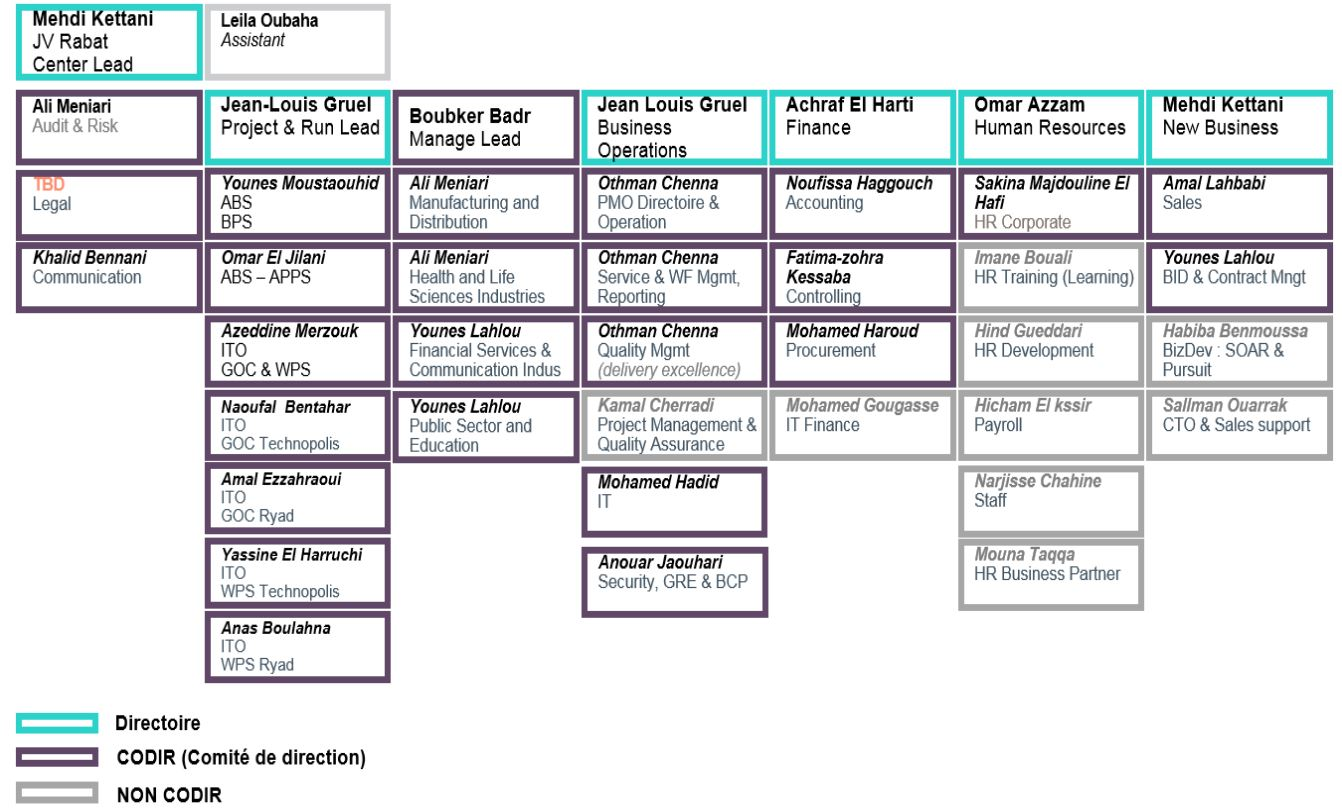
\includegraphics[scale=0.5,keepaspectratio]{Rapport de stage PFE chez DXC/figures/organigramme.jpg}
    \caption{Organigramme de DXC Technology}
\end{figure}
  
\end{description}


